
%template setup, made it adhere to UWA standards
\documentclass[12pt, a4paper]{article}
\usepackage{graphicx}
\usepackage{amsmath}
\usepackage{url}

%fix caption formatting
\usepackage[font=small,labelfont=bf]{caption}

%slightly modified UWA setup
\setlength{\oddsidemargin}{0.5cm}
\setlength{\evensidemargin}{0.5cm}
\setlength{\topmargin}{-1.6cm}
\setlength{\leftmargin}{0.5cm}
\setlength{\rightmargin}{0.5cm}
\setlength{\textheight}{24.00cm} 
\setlength{\textwidth}{15.0cm}
\parindent 0pt
\parskip 5pt
\pagestyle{plain}


%meta info
\title{The RNA Folding Problem}
\author{Max Ward \\
School of Computer Science \& Software Engineering \\
The University of Western Australia}
%let the date get auto generated

%author list formatter. not really needed here, but always nice to have
\newcommand{\namelistlabel}[1]{\mbox{#1}\hfil}
\newenvironment{namelist}[1]{%1
\begin{list}{}
    {
        \let\makelabel\namelistlabel
        \settowidth{\labelwidth}{#1}
        \setlength{\leftmargin}{1.1\labelwidth}
    }
  }{%1
\end{list}}



%-------------------------------------------------------------------------

\begin{document}


%title first!
\maketitle

\begin{abstract}
Ribonucleic Acid (RNA) is an important biological molecule with myriad functions. For example, it drives developmental processes, regulates the expression of genes, enables to synthesis of proteins, and catalyses important biological reactions. Because of this, algorithms for predicting RNA structures have been proposed as early as the 1970s. The problem they attempt to solve is called the RNA folding problem. In this report, I formally describe a simplified version of this problem, which I call the RNA bond problem. I show that this is equivalent to finding the maximum weight independent set of a circle graph, which is a common problem in VLSI design, bioinformatics, and register allocation for optimizing compilers. I then describe the Nussinov algorithm, which efficiently solves the RNA bond problem. Finally, I compare this algorithm to existing algorithms for solving the maximum weight independent set of a circle graph. It is noteworthy that nobody has recognized that these problems are equivalent, this highlights the issues associated with cliquing within scientific communities.
\end{abstract}


{\bf Keywords:} Ribonucleic acid, structure, prediction, empirical, comparison.

{\bf CR Classification:} J.3 Biology and genetics.

\clearpage

%\tableofcontents
%\listoffigures
%\clearpage

\section{Introduction}
Ribonucleic acid (RNA) is at the core of many biological processes. Traditionally it has been described as the messenger molecule of DNA, faithfully carrying code from DNA to the site of protein synthesis. However, in a recent landmark paper, Amaral et al. \cite{amaral2008eukaryotic} described our genome, and those of other eukaryotes, as being driven by a RNA machine. They noted that most of the eukaryote genome is transcribed into RNA, despite little of it coding for protein. It seems that much of our genome, originally called `junk DNA', codes for functional RNA molecules. These RNAs can interact with DNA, affecting gene expression. This allows DNA to essentially regulate itself. For example, Makeyev \& Maniati \cite{makeyev2008multilevel} reported that microRNAs affect the expression of genes by interfering with the translation of protein. They also argued that microRNAs, and other regulatory RNAs, explain the vast differences between organisms with similar genomes. To put this idea into perspective, we share roughly 90\% of our genes with the domestic cat \cite{pontius2007initial}. Mattick \cite{mattick2007new} has suggested that the process of development---from embryo to adult---is encoded in the interactions of such RNAs.

A widely held axiom is that chemical structure is tantamount to biological function. With increasingly important biological functions being associated with RNA, it is essential to accurately predict its structure. The purpose of this paper is to provide a survey of some widely used RNA structure prediction algorithms. In the interest of succinctness, I review only algorithms based on a thermodynamic model. Other algorithms often use machine learned parameters; these shall not be explored here as they represent fringe areas of research. In essence, all the algorithms I test take a single RNA primary sequence as input, and produce a predicted structure as output. I hypothesize that newer algorithms should have improved accuracy compared to older algorithms. In addition, I aim to empirically verify the time complexities of tested algorithms. The Zuker algorithm was the first thermodynamic algorithm to achieve usable prediction accuracy, and is the oldest algorithm I tested.

\subsection{The RNA Bond Problem}
\subsubsection{Description}
Before the RNA bond problem can be explained, some terminology and background information must be covered. A RNA molecule comprises a sequence of nucleotides connected in sequence. This is often described as a chain. The four RNA nucleotides are Adenosine (A), Uracil (U), Cytosine (C), and Guanine (G). Chemical bonds form between Adenosine and Uracil, such a bond is called an A-U bond. Other valid bonds are G-U, and G-C. Every bond causes the nucleotide chain to fold on itself. Successive folds lead to the complex, paper-clip like structures common to RNA molecules. For the sake of illustration, let use imagine a RNA nucleotide chain as being connected end to end, thus forming a circle. An example of this is shown visually in Figure \ref{my ass}. A valid bond is any chord crossing from one nucleotide to  another nucleotide, such that they form a chemically valid bond (A-U, G-C, or G-U). In addition, a valid bond must not cross any other chord in the circle. Finally, every bond has a weight, which indicates the strength of the bond. Examples of valid and invalid bonds can be seen in Figure \ref{my ass}. Given a RNA sequence, the RNA bond problem involves finding a set of valid bonds having maximum weight. In other words, we must find a collection of mutually valid chords such that their sum weight is maximized. I shall now outline an algorithm which solves this problem.

\begin{figure}
\begin{center}
\scalebox{0.27}{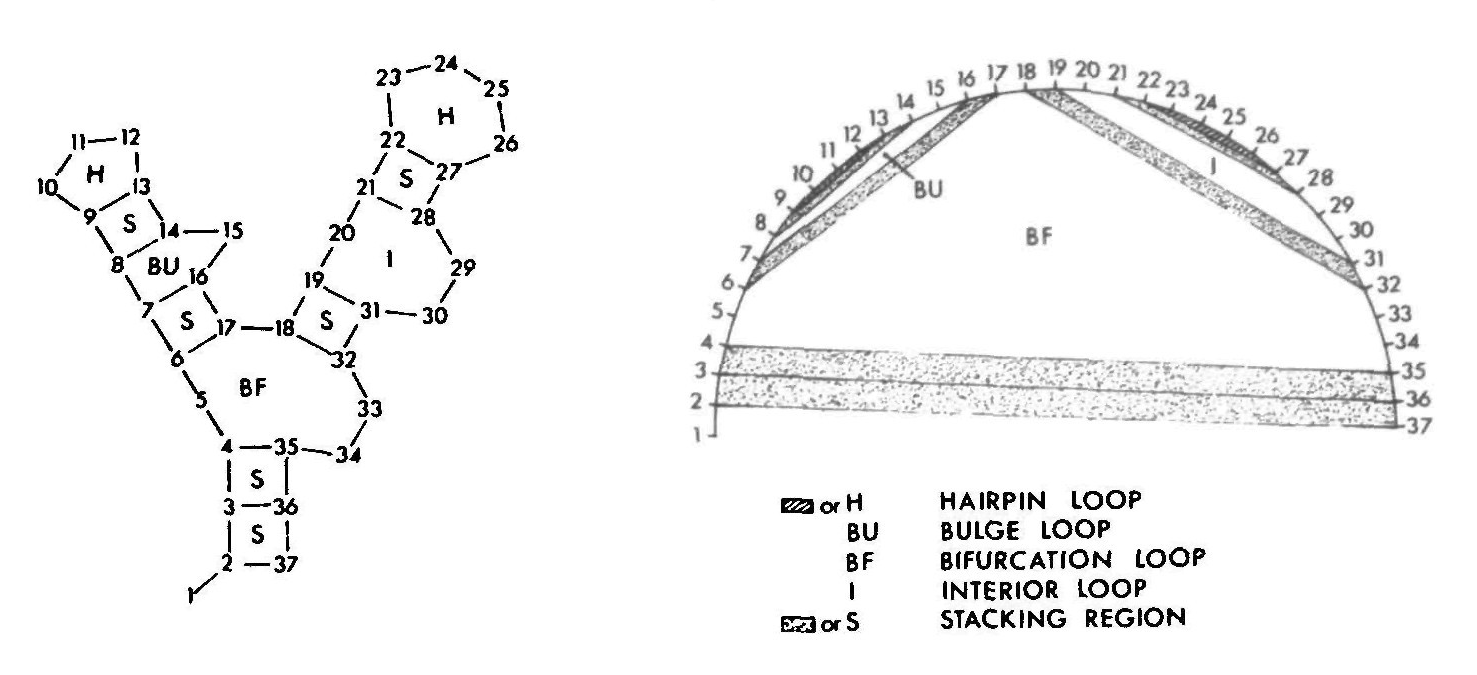
\includegraphics{figure4}}
\end{center}
\caption{Substructures used in the Zuker algorithm. On the left is a diagram of a RNA structure. On the right is the same structure laid out on a semi-circle. Bonds are represented as lines crossing the semi-circle. Taken from original
publication \cite{zuker1981optimal}.}
\label{fig:zuk_struct}
\end{figure}

\subsubsection{The Nussinov Algorithm}
In 1973 Nussinov \& someass described an algorithm that can efficiently find solutions to the RNA bond problem. However, this is not by design. The algorithm was originally introduced to solve the RNA folding problem. The intuition is that every bond increases the stability of the RNA's structure, so a structure with maximum bonds should be very stable. The Nussinov algorithm is no longer used in practice, as better algorithms now exist for solving the RNA folding problem. I describe it here only because it solves the RNA bond problem.

The nucleotides which make up a RNA sequence can be indexed from zero to $n-1$ where $n$ is the length of the RNA sequence. In addition, let the weight of a bond between nucleotides $i$ and $j$ be defined by $W(i,j)$. Also, the function $M(i,j)$ returns the solution to the RNA bond problem considering only nucleotides between $i$ and $j$ inclusive. This function is defined by the recurrence relation presented below.

\begin{align} \label{eq:nuss_eq}
	M(i, j) &= \max \left\lbrace A, B, C, D \right\rbrace \nonumber  \\
	A &= M(i, j-1) \nonumber \\
	B &= M(i+1, j) \nonumber \\
	C &= M(i+1, j-1) + W(i, j) \nonumber \\
	D &= \max \left\lbrace M(i, k) + M(k+1, j) \right\rbrace \: for \: all \: k \: where \: i < k < j \nonumber	\\
\end{align}

The recurrence relation in Equation \ref{eq:nuss_eq} describes the Nussninov algorithm. It can be used to solve the RNA bond problem by calling $M(0, \: \texttt{RNA\_Length}-1)$. The first two cases ($A$ and $B$) find the score associated with not allowing the bases corresponding to indexes $i$ and $j$ to bond. Case $C$ conversely determines the score given that $i$ and $j$ are bonded. The final case $D$ computes the score associated with a bifurcation. A bifurcation is the decomposition of RNA into two separate structures. This recurrence relation is solved using dynamic programming. As such, it implies a $O(N^3)$
worst case time complexity and a $O(N^2)$ space complexity, as a $O(N^2)$ state space (all combinations of $i$ and $j$) is explored
with a linear time recurrence relation.


\section{Maximum Weight Independent Sets and Circle Graphs}
\subsection{Description}
An independent set of a graph is any collection of vertices such that none share an edge. The maximum weight independent set of a graph requires that vertices have weights. It is defined as any independent set such that the sum weight of vertices is maximal. A circle graph is a special kind of graph derived from a circle diagram. A circle diagram is easy to visualize. Given a circle, a circle diagram also has a collection of chords cross the inside edge of this circle. A circle graph is derived from a circle diagram using a simple procedure. Every chord is represented by a vertex. Two vertices share an edge if and only if the chords they represent intersect in the circle diagram. This is best explained using a diagram, as such, I have included Figure \ref{myass}. Finding the maximum weight independent set of a circle graph is equivalent to finding a set of non-intersecting chords with maximum sum weight in the circle diagram.

Finding the maximum weight independent set of a circle graph has several practically important applications. For example blah blah blah.

\subsection{Graphs and RNA}
I now wish to point out that the RNA bond problem is isomorphic to finding the maximum weight independent set of a circle graph. This is the core observation of this report. If we imagine an RNA joined end to end in a circle, and all of the possible valid bonds represented as chords across the circle, the solution to the RNA bond problem is any subset of chords that do not intersect, and which has maximum sum weight. This is, by definition, also a maximum weight independent set. As such, the Nussinov algorithm finds the maximum weight independent set of a circle graph.

Borrowing terminology from literature on graph theory, I shall refer to the number of distinct points on a circle graph as $n$, and the number of chords as $m$. Thus, we say that the Nussinov algorithm takes $O(n^3)$ time. The Nussinov algorithm was published in 1978. The most optimal algorithm for finding the maximum weight independent set of a circle graph at the time required $O(m^3)$ time, and was discovered in 1973. Clearly this is inferior to the Nussinov algorithm, as $m$ is bounded from below by $2 \times n$ when every end point is unique. It wasn't until 2003 that a clearly better algorithm was found. This algorithm required $O(md)$ time, and was discovered by Valentino \ref{dfg}. Note that $d$ represents the density of the graph, but the precise complexity analysis is not important for this discussion. Despite the Nussinov algorithm being an asymptotically superior algorithm for 20 years, it was never used outside of RNA research.


\section{Conclusions}
I have briefly introduced the RNA folding problem. Following this, a precise definition of a simpler problem, the RNA bond problem, was described. The Nussinov algorithm is an relatively simple and reasonably efficient solution to this problem. In addition, I have showed that the RNA bond problem, and finding the maximum weight independent set of a circle graph, is equivalent. Thus the Nussinov algorithm solves both problems. In addition, it is more optimal than the other algorithms that solve the same problem at the time of its publication. However, this has note been recognized until now. I submit that this illustrates the danger with over specialization within scientific communities. I also conjecture that this situation would have been avoided with a more holistic approach to research. All
knowledge is valuable; insular research has no place in the advancement of science


%let bibtex do all the hard work
\bibliographystyle{plain}
\bibliography{assignment_one}


\end{document}

